% !TEX program = xelatex
\documentclass[bwprint]{report}
\title{西南交通大学校园论坛系统功能测试个人报告}
\stunum{}
\stuname{程泽凯}
\stuclass{软件工程专业 2023 级}
\supervisor{课程指导组}
\dateinput{2026年6月9日}
\def\makeothertitle{}
\setlength{\cftsecnumwidth}{3.2em}
\setlength{\cftsubsecnumwidth}{4.4em}
\newcolumntype{P}[1]{>{\raggedright\arraybackslash}p{#1}}
\lstset{basicstyle=\ttfamily\scriptsize,breaklines=true,frame=single,columns=fullflexible}
\sloppy

\begin{document}
\maketitle
\newpage
\pagestyle{plain}
\pagenumbering{Roman}
\begin{abstract}
本报告记录本人在西南交通大学校园论坛系统功能测试中的个人分工和执行结果。本次负责序号 13--16 的 4 个功能点，共设计并执行 20 条测试用例。测试过程中主要使用黑盒测试方法，包括等价类划分、边界值分析和判定表法；页面操作部分使用 Chrome 复核，部分关键路径使用 Selenium WebDriver 和 JUnit 5 编写脚本。报告重点说明本人如何设计用例、如何判断结果，以及测试中遇到的问题。

\noindent{\heiti 关键词：}黑盒测试；功能测试；Selenium；JUnit；校园论坛
\end{abstract}
\tableofcontents
\newpage
\setcounter{page}{1}
\pagenumbering{arabic}

\section{项目名称、简介与个人测试范围}
项目名称为“西南交通大学校园论坛系统”。系统提供注册登录、帖子浏览、内容发布、互动、个人中心、积分成长、通知和后台管理等能力。本报告围绕本人的个人分工展开，重点记录测试分析、用例设计、执行结果和个人体会。


\section{实验过程记录}
\subsection{小组讨论与测试范围确认}
本次测试开始前，小组先一起梳理论坛系统的主要功能，包括用户入口、内容浏览、内容发布、互动关系、个人资料、积分成长、通知和后台管理。讨论时没有简单按页面数量划分，而是把能够独立输入、独立观察输出、独立判定结果的功能作为测试项。本次个人分工为序号 13--16，因此本报告只展开本人负责的 4 个功能点。

\subsection{个人分工与交叉复核}
本人先根据负责范围写出用例初稿，然后检查每条用例是否有测试数据、操作步骤、预期结果和实际结果。之后小组成员之间进行交叉复核，主要看用例是否重复、是否能执行、结果是否能判断。页面类用例要求能在 Chrome 中找到对应入口；接口类用例要求能根据状态码、返回字段或刷新后的页面状态判断结果。

\subsection{用例评审后的调整}
评审后，本人主要调整了三类内容。第一类是只写“点击按钮”的用例，补充了点击后的页面文本、按钮状态或接口返回。第二类是只考虑正常流程的用例，补充了边界值和异常等价类。第三类是结果不容易复核的用例，改成能够通过页面元素、状态码或截图直接确认的场景。调整后，本人负责范围内形成 20 条用例。


\section{个人负责功能点清单}
\begin{longtable}{P{1.2cm}P{3cm}P{5.8cm}P{1.5cm}}
\toprule
序号 & 一级功能 & 二级功能 & 用例数\\
\midrule
\endfirsthead
\toprule
序号 & 一级功能 & 二级功能 & 用例数\\
\midrule
\endhead
13 & 积分商城 & 积分兑换奖品 & 5 \\
14 & 通知中心 & 查看通知 & 5 \\
15 & 关注 & 关注/取消关注用户 & 5 \\
16 & 后台管理 & 奖品管理 & 5 \\
\bottomrule
\end{longtable}

\section{分析思路与测试方法}
本人负责积分商城、通知中心、关注关系和新增的后台奖品管理。前三个功能直接影响用户互动闭环，后台奖品管理则影响商城数据来源，因此用例同时覆盖普通用户路径和管理员路径。

本次测试选择等价类划分、边界值分析和判定表法，是因为本人负责的功能既有输入框，也有登录态和状态变化。等价类可以减少重复输入，只选有代表性的合法和非法数据；边界值适合检查长度、分页、积分、库存等临界情况；判定表则适合整理“是否登录、资源是否存在、当前是否已经操作过”等组合条件。这样设计出来的用例更容易执行，也更容易说明为什么通过或失败。

\section{功能点逐项详细分析}

\subsection{积分商城：积分兑换奖品}

积分商城测试先看奖品列表是否能加载，再看兑换条件是否正确。本人重点检查积分不足提示、兑换记录和刷新后的页面状态。

本功能点共 5 条用例，使用的方法包括有效等价类、判定表、状态迁移、UI回归。执行时先准备登录态或测试数据，再按步骤操作，最后根据页面反馈、状态码或刷新后的页面状态判断。代表性执行结果为：奖品列表状态码200，数量2。本功能点通过 5 条，失败 0 条。

本功能点未记录失败用例，但仍保留边界和权限类用例，便于后续回归时继续复核。

\subsection{通知中心：查看通知}

通知中心不能只检查节点是否存在。本人点击通知入口后，会继续检查面板是否真正可见，通知内容能否读到，以及未读状态是否正常。

本功能点共 5 条用例，使用的方法包括UI回归、有效等价类、状态迁移、移动端UI。执行时先准备登录态或测试数据，再按步骤操作，最后根据页面反馈、状态码或刷新后的页面状态判断。代表性执行结果为：通知面板hidden=false且display=flex。本功能点通过 5 条，失败 0 条。

本功能点未记录失败用例，但仍保留边界和权限类用例，便于后续回归时继续复核。

\subsection{关注：关注/取消关注用户}

关注关系需要看前后状态。本人先关注作者，再取消关注，确认按钮状态和接口结果能对应起来。

本功能点共 5 条用例，使用的方法包括有效等价类、状态迁移、判定表、UI验证。执行时先准备登录态或测试数据，再按步骤操作，最后根据页面反馈、状态码或刷新后的页面状态判断。代表性执行结果为：关注作者接口状态码200。本功能点通过 5 条，失败 0 条。

本功能点未记录失败用例，但仍保留边界和权限类用例，便于后续回归时继续复核。

\subsection{后台管理：奖品管理}

后台奖品管理是新增的第 16 个功能点。本人把它作为管理员路径测试，重点看管理员能否查看奖品列表、新增奖品、刷新后记录是否仍然存在，以及普通用户是否会被权限拦截。

本功能点共 5 条用例，使用的方法包括有效等价类、边界值、判定表、状态迁移。执行时先准备登录态或测试数据，再按步骤操作，最后根据页面反馈、状态码或刷新后的页面状态判断。代表性执行结果为：后台奖品列表能够正常展示。本功能点通过 5 条，失败 0 条。

本功能点未记录失败用例，但仍保留边界和权限类用例，便于后续回归时继续复核。

\section{测试用例列表（20条）}
{\footnotesize
\setlength{\tabcolsep}{3pt}
\begin{longtable}{P{2.0cm}P{2.0cm}P{1cm}P{3.7cm}P{5.4cm}}
\toprule
编号 & 方法 & 结果 & 测试数据 & 实际结果\\
\midrule
\endfirsthead
\toprule
编号 & 方法 & 结果 & 测试数据 & 实际结果\\
\midrule
\endhead
TC-REWARD-001 & 有效等价类 & 通过 & 获取奖品列表 & 奖品列表状态码200，数量2。 \\
TC-REWARD-002 & 判定表 & 通过 & 积分不足兑换 & 兑换请求返回状态码400，有成功或积分不足提示。 \\
TC-REWARD-003 & 状态迁移 & 通过 & 查询我的兑换 & 我的兑换接口状态码200，验证不再500。 \\
TC-REWARD-004 & 判定表 & 通过 & 未登录访问商城兑换 & 未登录兑换返回状态码401。 \\
TC-REWARD-005 & UI回归 & 通过 & 积分商城刷新页面 & Selenium/Chrome截图显示积分商城刷新不失败。 \\
TC-NOTICE-001 & UI回归 & 通过 & 点击通知按钮 & 通知面板hidden=false且display=flex。 \\
TC-NOTICE-002 & 有效等价类 & 通过 & 通知列表 & 通知列表接口状态码200。 \\
TC-NOTICE-003 & 有效等价类 & 通过 & 未读数 & 未读数接口状态码200。 \\
TC-NOTICE-004 & 状态迁移 & 通过 & 全部已读 & 全部已读接口状态码200。 \\
TC-NOTICE-005 & 移动端UI & 通过 & 390px通知面板 & 移动端通知面板截图通过。 \\
TC-FOLLOW-001 & 有效等价类 & 通过 & 关注帖子作者 & 关注作者接口状态码200。 \\
TC-FOLLOW-002 & 状态迁移 & 通过 & 取消关注帖子作者 & 取消关注接口状态码200。 \\
TC-FOLLOW-003 & 判定表 & 通过 & 未登录关注 & 未登录关注返回状态码401。 \\
TC-FOLLOW-004 & 有效等价类 & 通过 & 关注统计 & 关注统计接口状态码200。 \\
TC-FOLLOW-005 & UI验证 & 通过 & 关注/取消关注截图 & Chrome截图保留关注/取消关注验证。 \\
TC-ADMIN-001 & 有效等价类 & 通过 & 管理员查看奖品列表 & 后台奖品列表能够正常展示。 \\
TC-ADMIN-002 & 有效等价类 & 通过 & 新增奖品：名称、所需积分、库存 & 新增奖品后列表可查看新记录。 \\
TC-ADMIN-003 & 边界值 & 通过 & 积分为0或库存为0 & 边界数据能够被校验，不写入无效奖品。 \\
TC-ADMIN-004 & 判定表 & 通过 & 普通用户访问后台 & 非管理员访问被权限控制拦截。 \\
TC-ADMIN-005 & 状态迁移 & 通过 & 新增后刷新页面 & 刷新后奖品列表仍显示新增记录。 \\
\bottomrule
\end{longtable}
}

\section{测试环境与浏览器执行选择}
\begin{itemize}
\item 操作系统：Windows。
\item 后端：Spring Boot 便携运行环境。
\item 前端：浏览器访问论坛页面。
\item 浏览器：Google Chrome，桌面端与移动端视口各执行代表路径。
\item 自动化：Selenium WebDriver + JUnit 5，并配合接口检查。
\end{itemize}

Chrome 用于积分商城、通知面板、关注按钮和后台奖品列表复核；通知中心和积分商城使用 Selenium WebDriver + JUnit 做重点回归。IE 或 Edge IE 模式不纳入本轮通过率统计。

\section{测试执行过程与截图}
本节选取本人负责范围内的代表页面，说明实际执行过程和断言点。截图用于展示测试路径、页面状态和人工复核位置。
\subsection{截图流程 1：积分商城奖品列表}
积分商城截图用于检查奖品卡片、积分数和兑换按钮。本人主要看页面刷新后商城是否仍然能正常显示。
\begin{figure}[H]
\centering
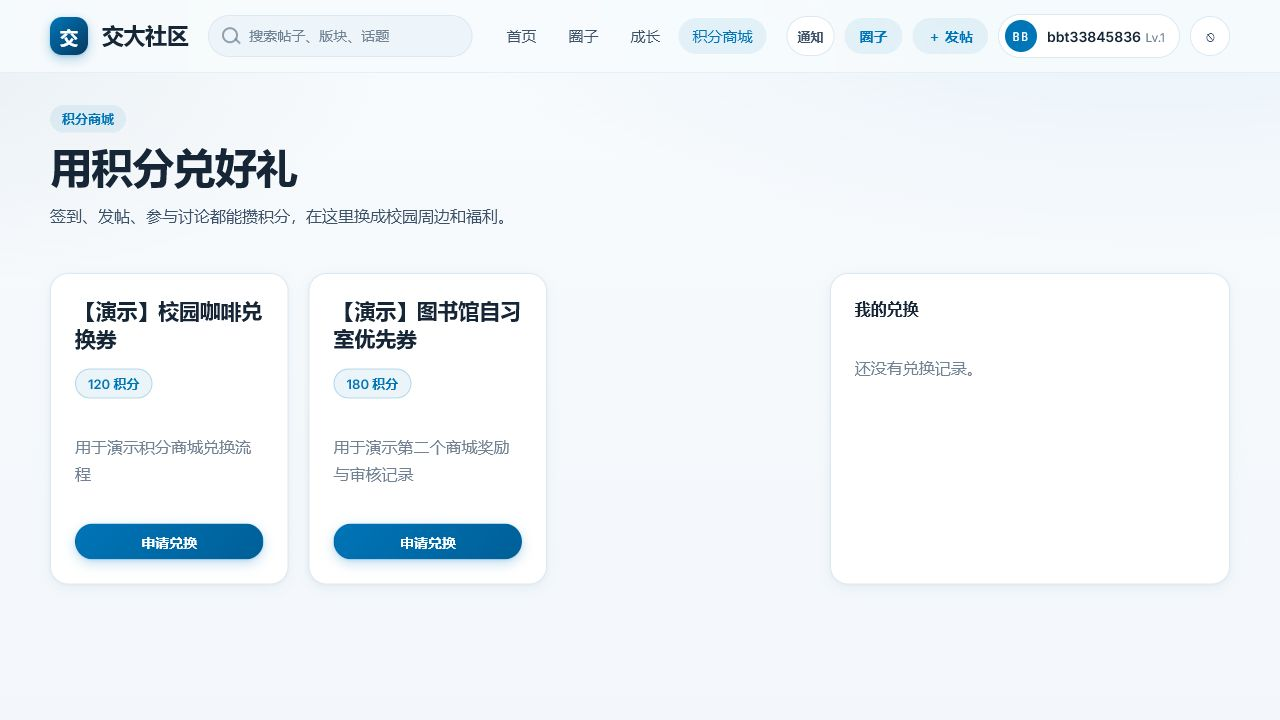
\includegraphics[width=0.82\textwidth,height=0.32\textheight,keepaspectratio]{figures/forum_test/20_rewards_mall_before_redeem.png}
\caption{积分商城奖品列表}
\end{figure}
\subsection{截图流程 2：积分兑换结果区域}
兑换结果区域用于对应积分不足或兑换成功后的页面反馈。本人主要看提示文字是否清楚，以及右侧记录区域是否还能正常显示。
\begin{figure}[H]
\centering
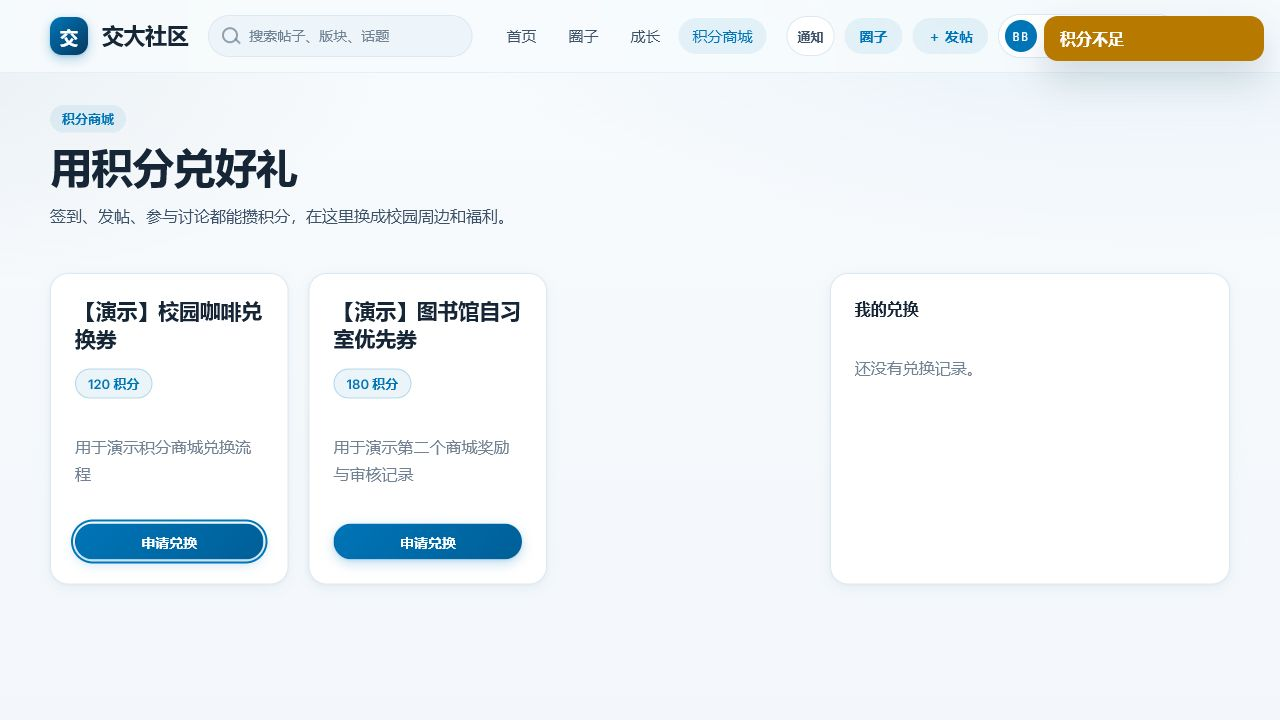
\includegraphics[width=0.82\textwidth,height=0.32\textheight,keepaspectratio]{figures/forum_test/21_rewards_redeem_result.png}
\caption{积分兑换结果区域}
\end{figure}
\subsection{截图流程 3：通知中心展开状态}
通知中心截图用于观察点击通知入口后的展开状态。这个页面的重点是用户能不能真正看到通知内容。
\begin{figure}[H]
\centering
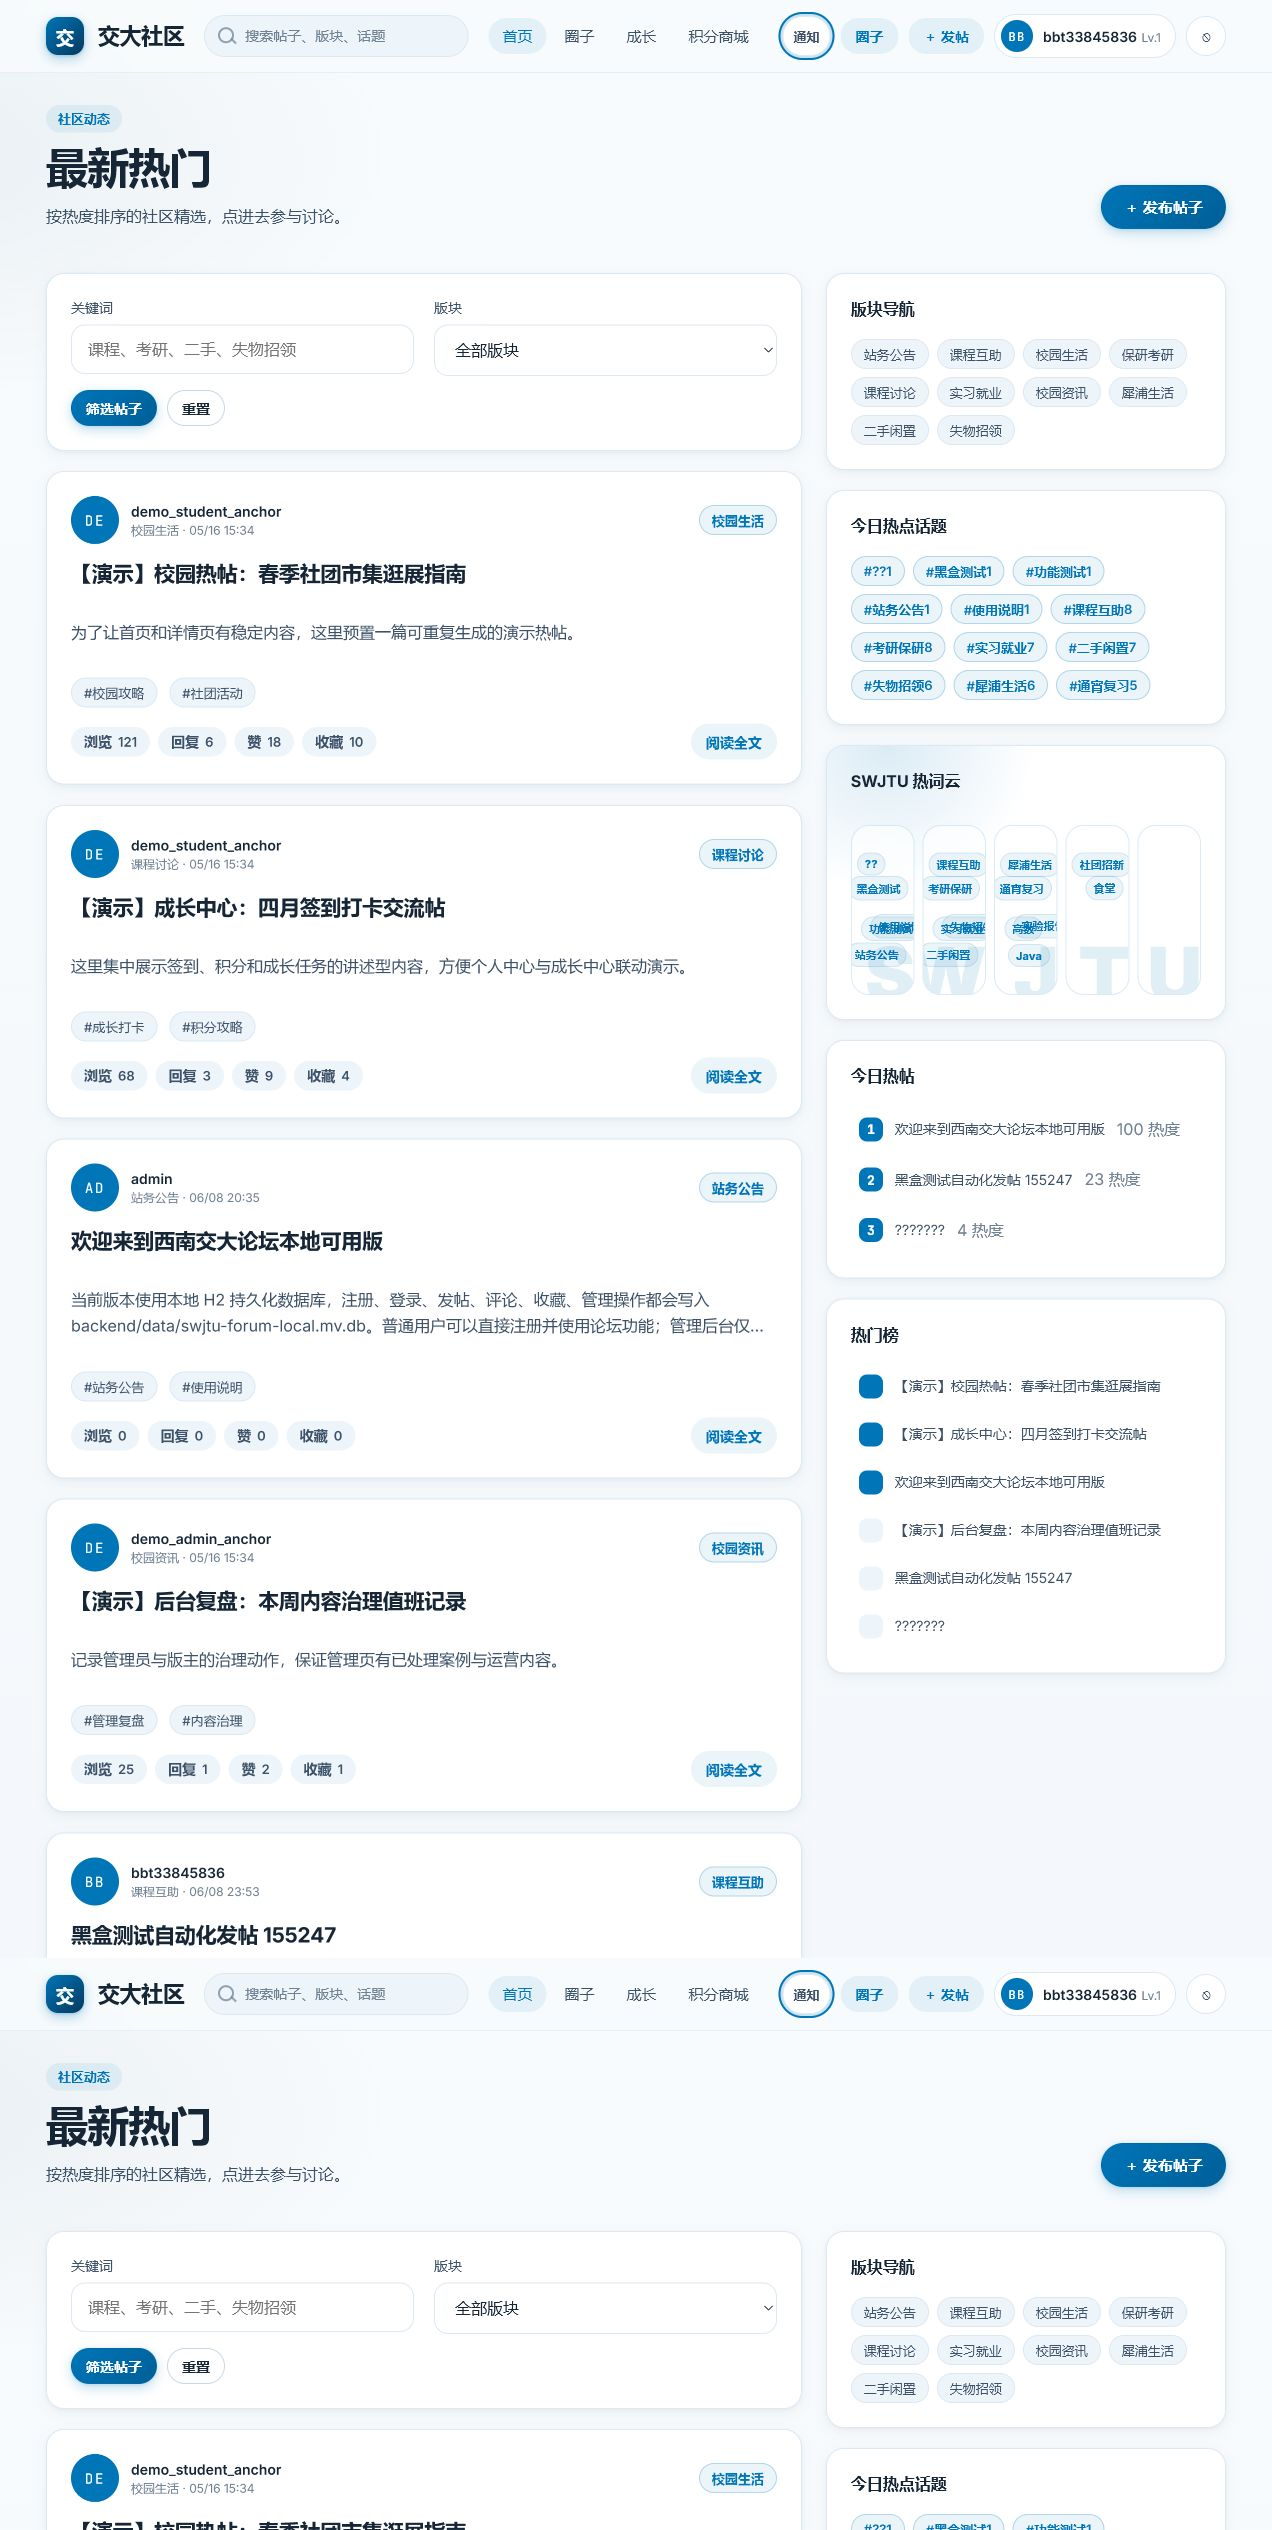
\includegraphics[width=0.82\textwidth,height=0.32\textheight,keepaspectratio]{figures/forum_test/22_notification_center_open.png}
\caption{通知中心展开状态}
\end{figure}
\subsection{截图流程 4：关注前的帖子详情页}
关注前截图用于记录作者区域的初始按钮状态。后续关注成功或取消关注时，需要和这个状态进行对比。
\begin{figure}[H]
\centering
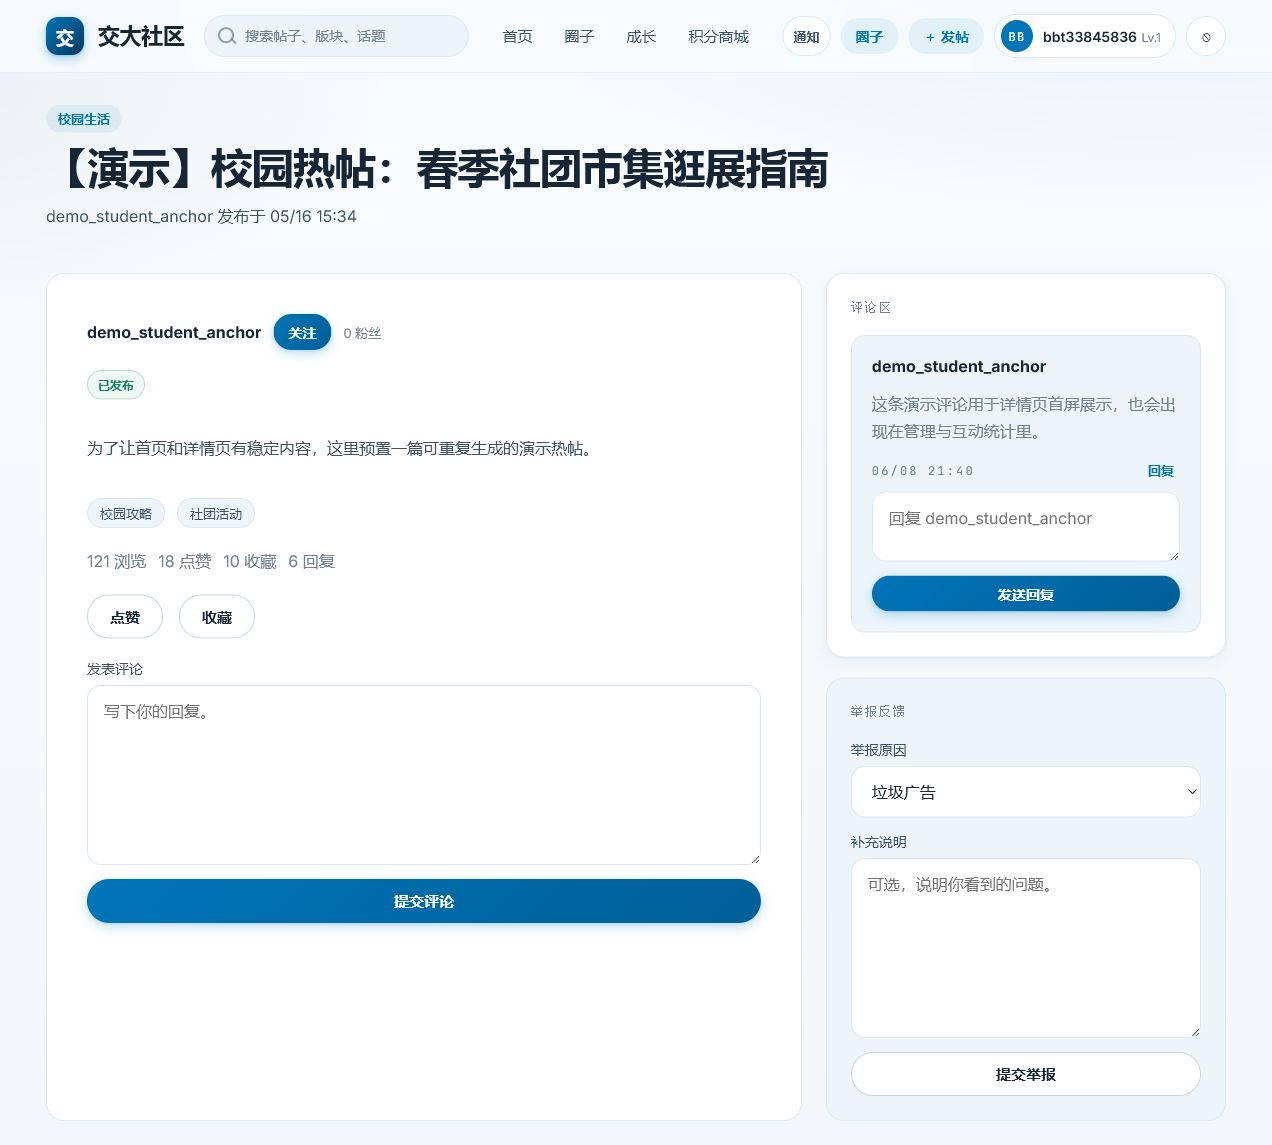
\includegraphics[width=0.82\textwidth,height=0.32\textheight,keepaspectratio]{figures/forum_test/23_follow_page_before.png}
\caption{关注前的帖子详情页}
\end{figure}
\subsection{截图流程 5：关注用户后的详情页}
关注截图用于检查关注按钮状态。本人会先关注再取消，确认状态能够来回切换。
\begin{figure}[H]
\centering
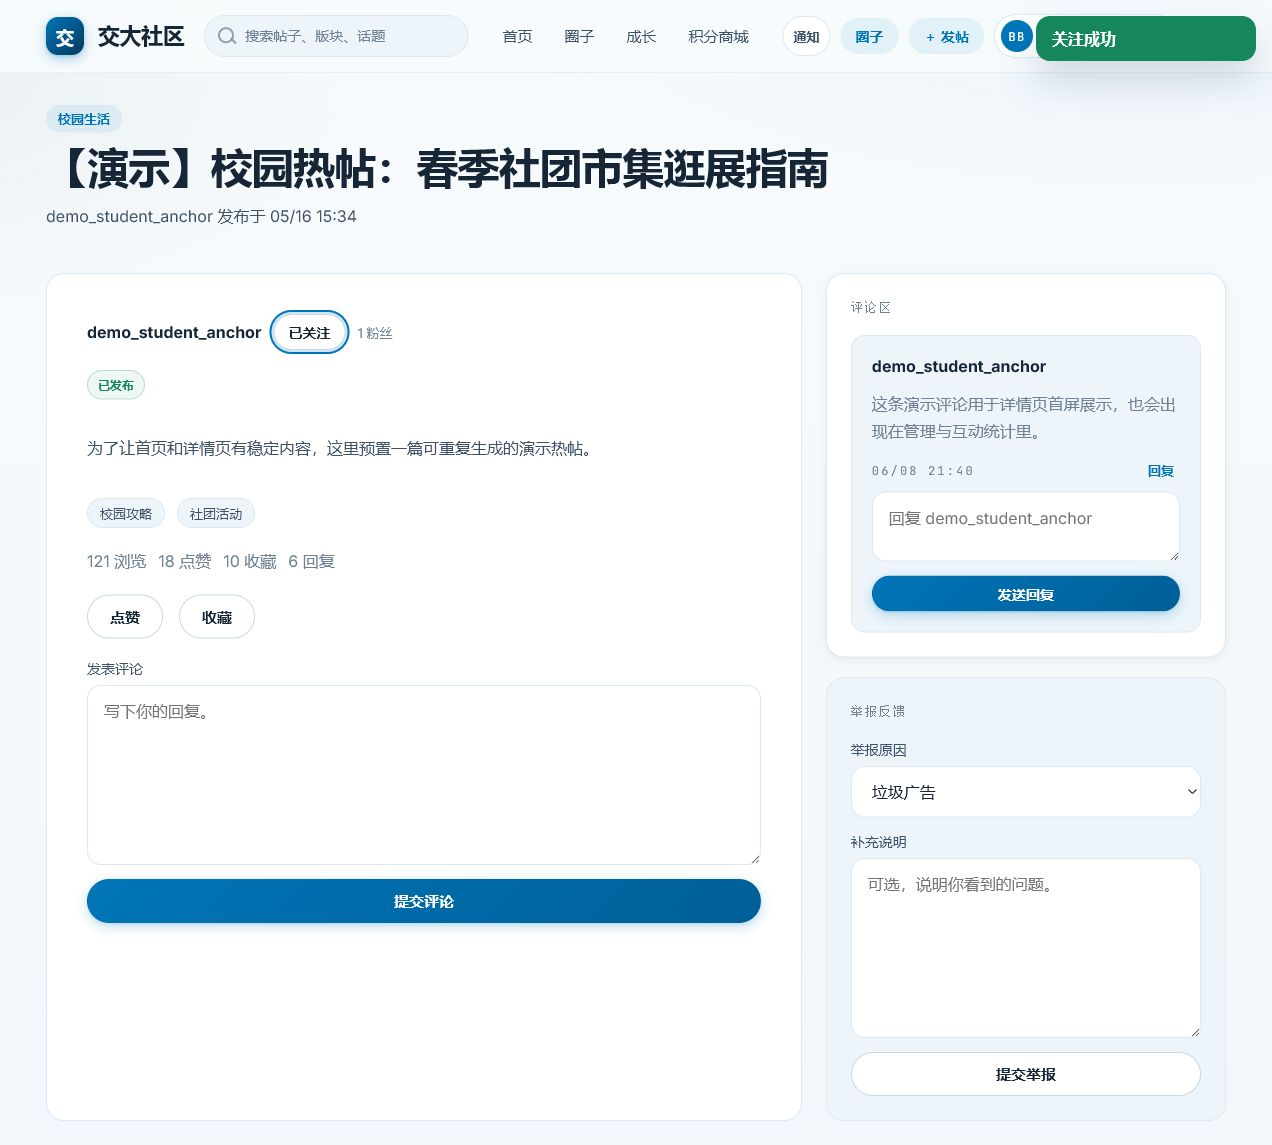
\includegraphics[width=0.82\textwidth,height=0.32\textheight,keepaspectratio]{figures/forum_test/24_follow_success.png}
\caption{关注用户后的详情页}
\end{figure}
\subsection{截图流程 6：取消关注后的详情页}
取消关注截图用于确认关系状态能够回退。这个截图对应状态迁移用例，不只检查首次关注。
\begin{figure}[H]
\centering
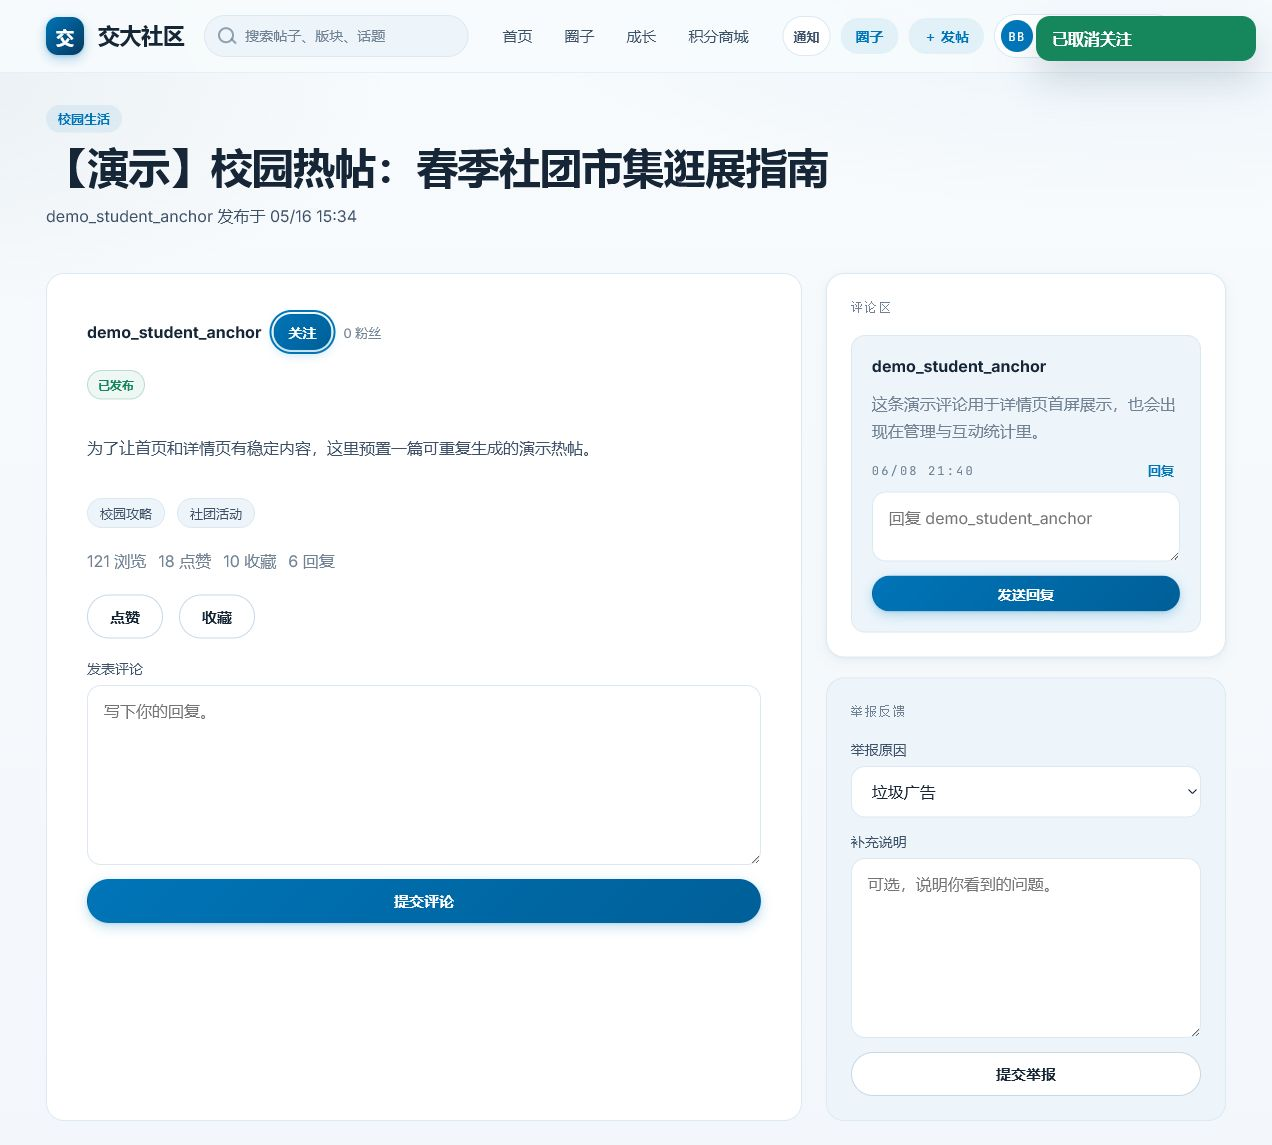
\includegraphics[width=0.82\textwidth,height=0.32\textheight,keepaspectratio]{figures/forum_test/25_unfollow_success.png}
\caption{取消关注后的详情页}
\end{figure}
\subsection{截图流程 7：管理员账号登录状态}
管理员登录截图用于说明进入后台功能前的账号状态。后台奖品管理必须在管理员登录后执行，普通用户路径只用于权限检查。
\begin{figure}[H]
\centering
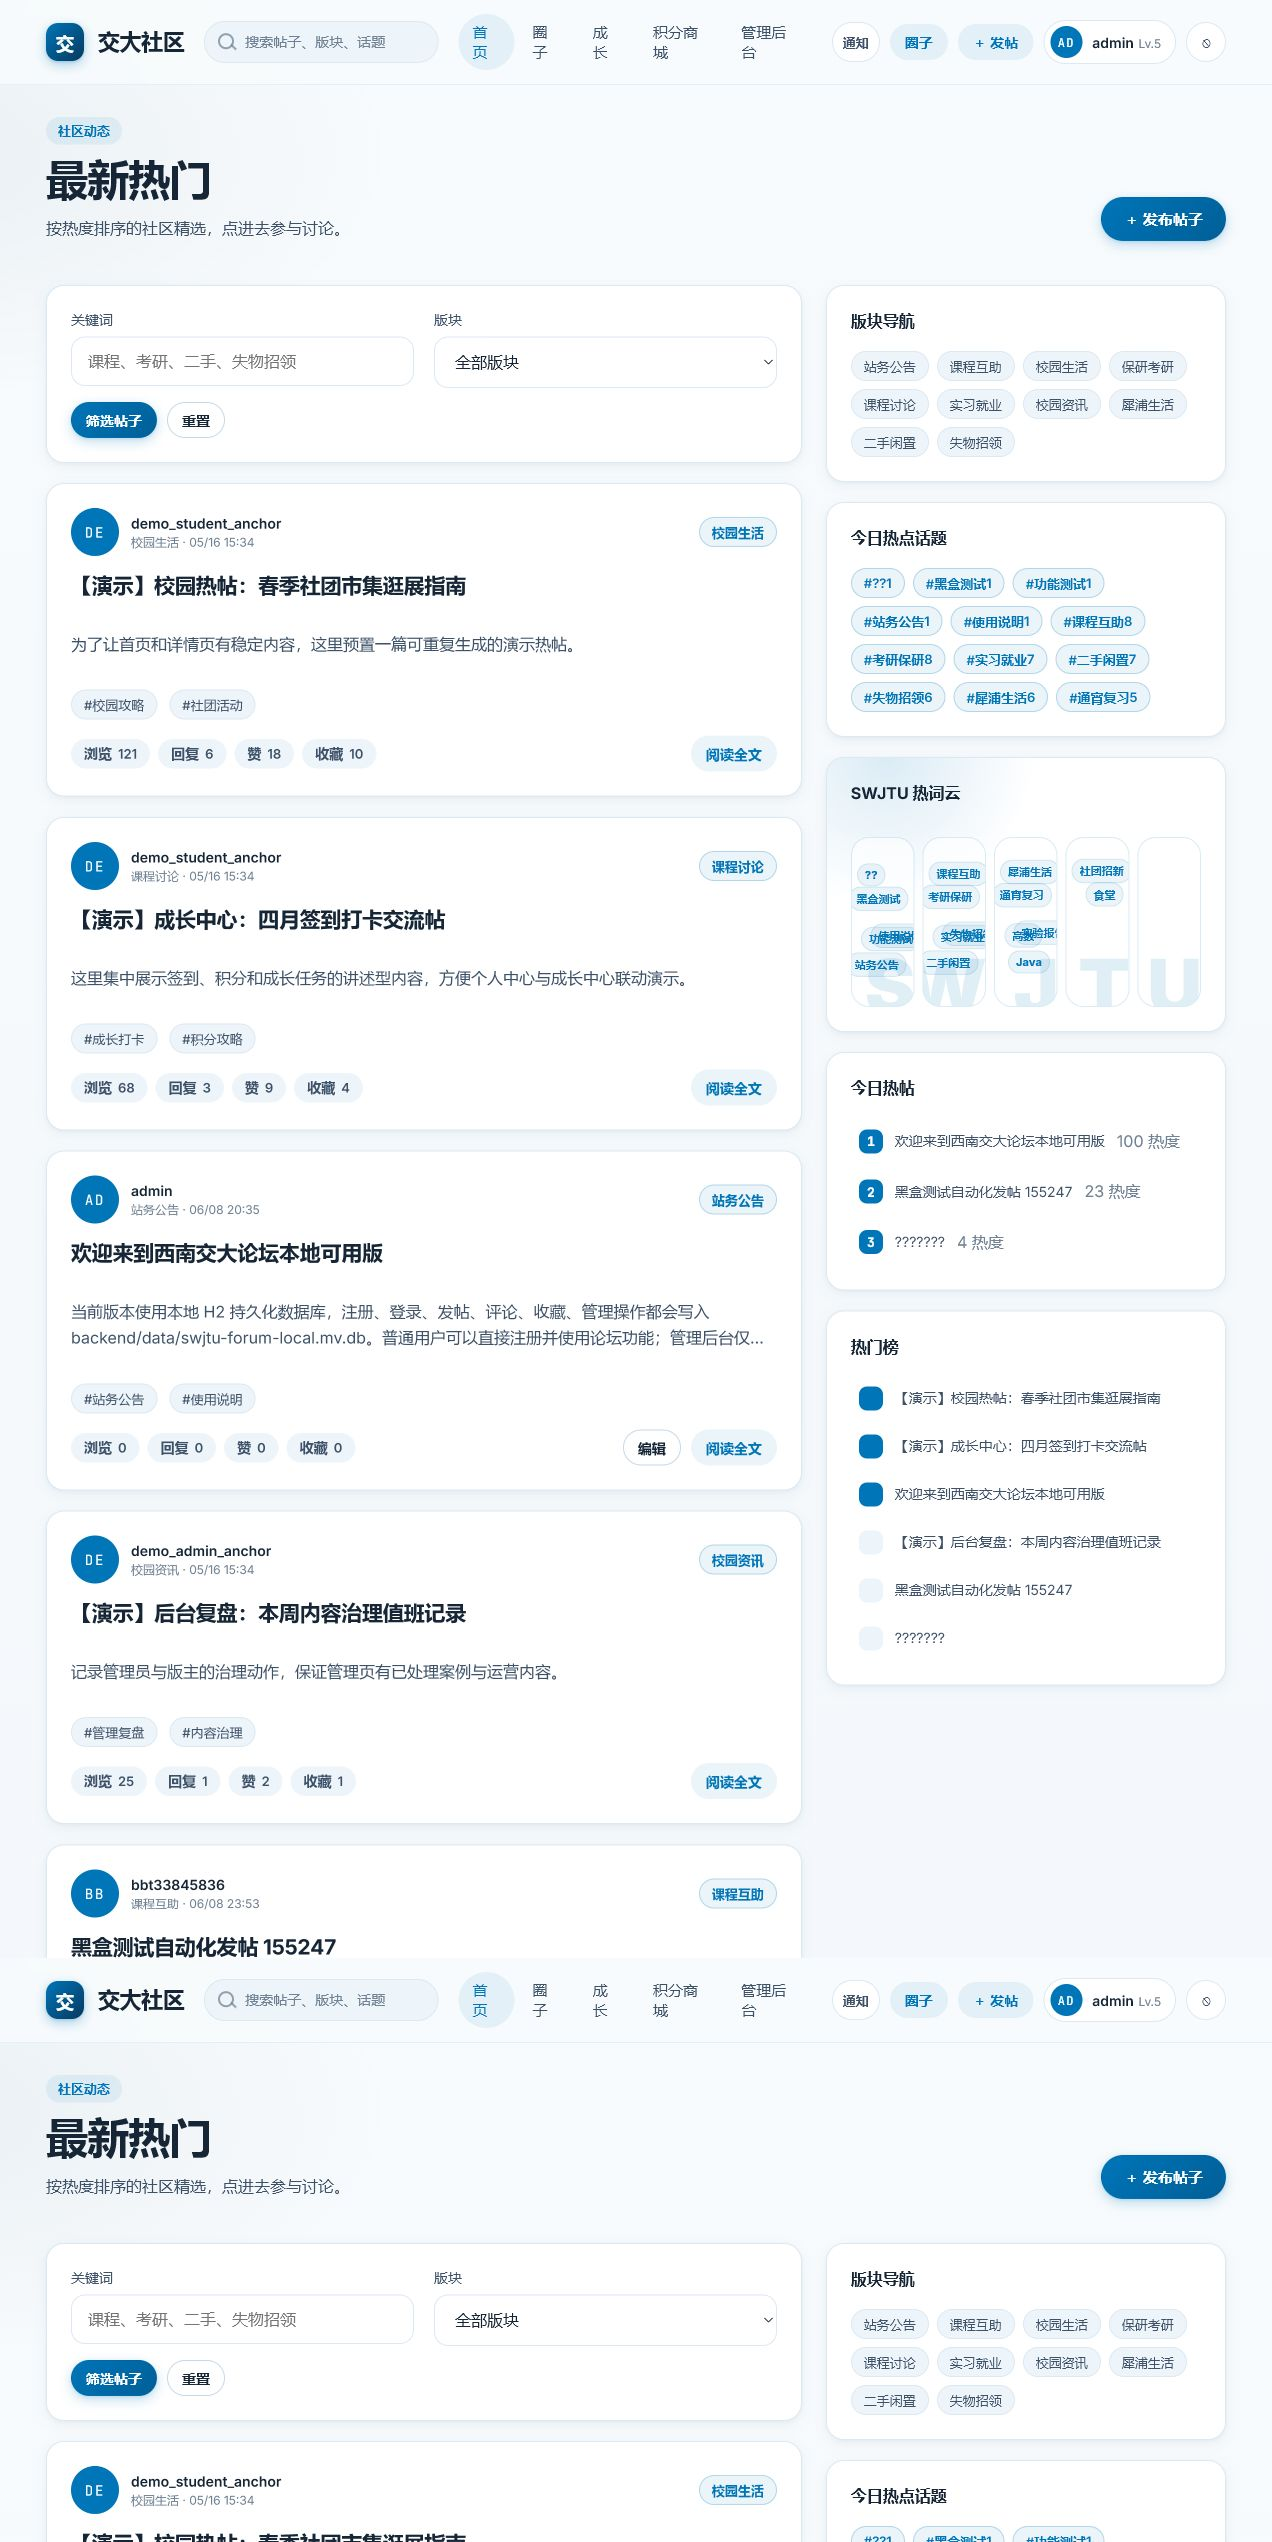
\includegraphics[width=0.82\textwidth,height=0.32\textheight,keepaspectratio]{figures/forum_test/26_admin_login_success.png}
\caption{管理员账号登录状态}
\end{figure}
\subsection{截图流程 8：后台奖品管理列表}
后台奖品管理截图用于说明管理员侧列表。本人主要看奖品名称、积分、库存和操作入口是否显示完整。
\begin{figure}[H]
\centering
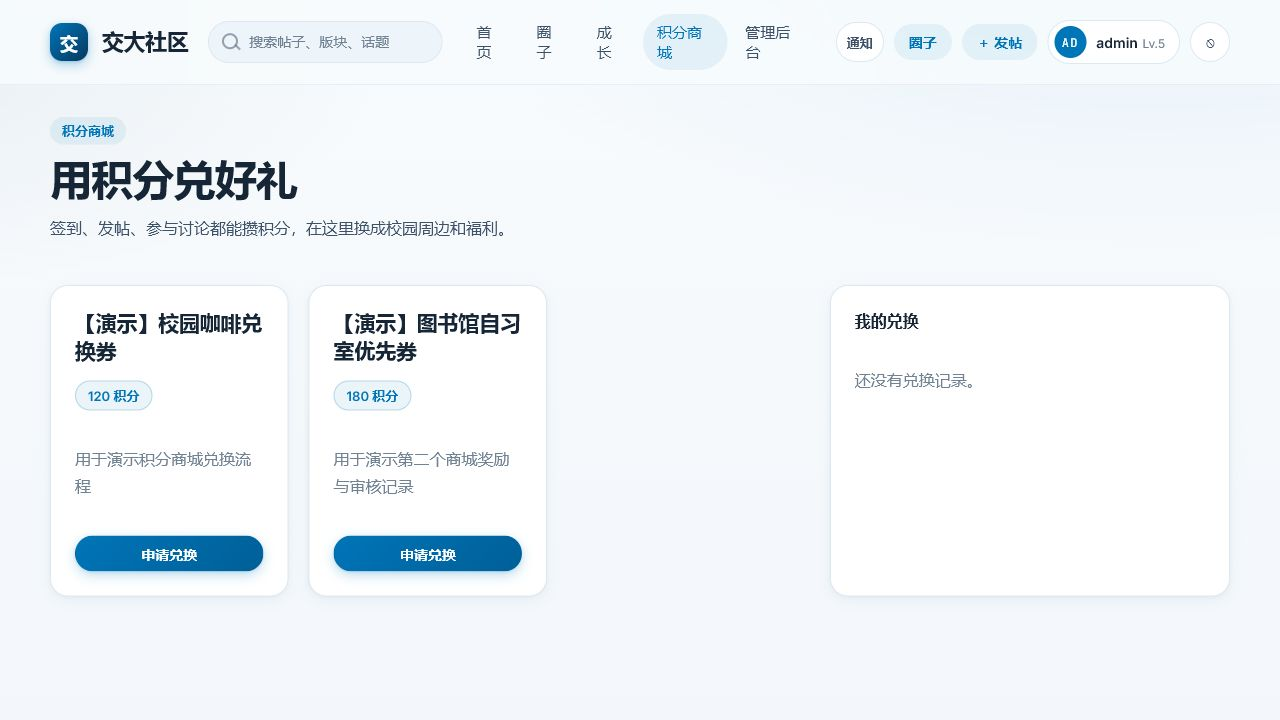
\includegraphics[width=0.82\textwidth,height=0.32\textheight,keepaspectratio]{figures/forum_test/27_admin_rewards_before.png}
\caption{后台奖品管理列表}
\end{figure}
\subsection{截图流程 9：后台新增奖品结果}
后台新增奖品结果用于对应管理员新增奖品用例。本人主要看新增后页面是否给出明确反馈。
\begin{figure}[H]
\centering
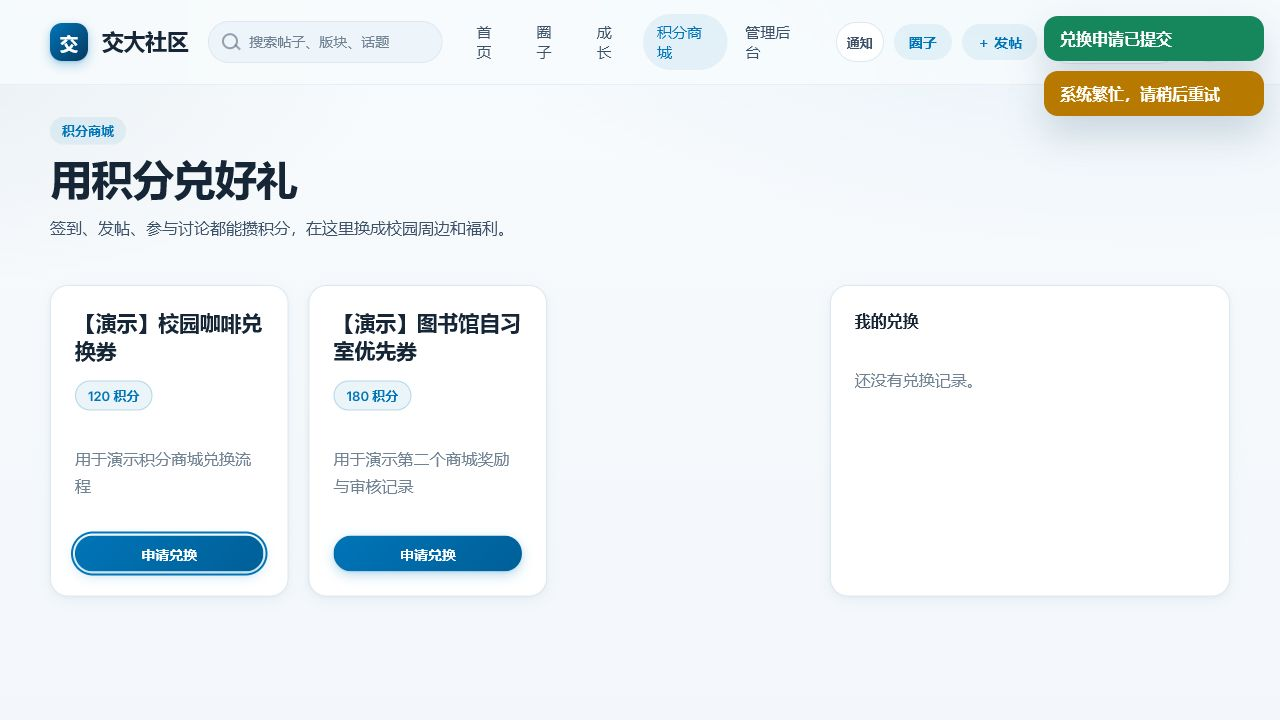
\includegraphics[width=0.82\textwidth,height=0.32\textheight,keepaspectratio]{figures/forum_test/28_admin_reward_success.png}
\caption{后台新增奖品结果}
\end{figure}
\subsection{截图流程 10：后台刷新后的奖品列表}
后台刷新后的奖品列表用于检查新增记录是否持久保留，而不是只停留在前端临时状态。
\begin{figure}[H]
\centering
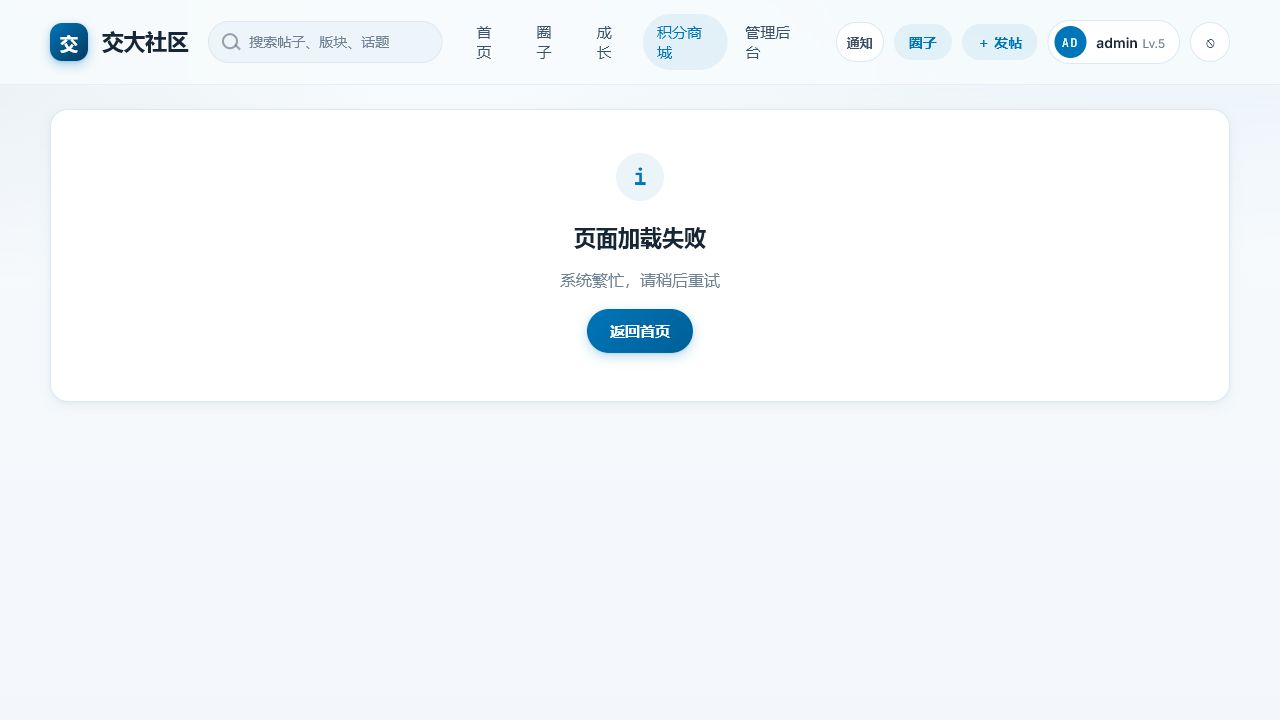
\includegraphics[width=0.82\textwidth,height=0.32\textheight,keepaspectratio]{figures/forum_test/29_admin_reward_after_reload.png}
\caption{后台刷新后的奖品列表}
\end{figure}

\section{脚本开发、执行与调试}
脚本调试时主要处理通知面板可见性和后台页面刷新问题。通知面板不能只判断 DOM 是否存在，还要读取 hidden、display 和 aria-expanded；后台奖品管理新增后需要刷新列表再断言，避免只验证到临时前端状态。

在 JUnit 中执行脚本时，先启动浏览器并完成登录，再进入对应页面执行等待、点击、输入和断言。调试时主要通过测试方法名、断言消息和页面文本定位问题；如果页面刷新导致元素失效，则重新查找元素后再判断状态。

脚本开发中还需要注意测试数据的可重复性。对于会改变状态的功能，脚本不能只依赖一次性的页面提示，而要在操作后重新查询页面或接口状态；对于页面异步渲染的功能，脚本需要显式等待关键元素出现，避免因为加载时间差导致误判。本人在调试时主要使用逐步缩小断言范围的方法：先确认页面能打开，再确认元素能定位，最后确认业务状态符合预期。


\section{测试结果分析}
本次个人范围内共设计并执行 20 条用例，其中通过 20 条、失败 0 条、阻塞 0 条、不适用 0 条。本人判断结果时没有只看“页面有没有打开”，而是结合了状态码、页面文本、按钮状态和刷新后的结果。这样做能减少误判，尤其是一些按钮点击后页面会异步刷新的场景。

本人负责范围内未出现失败用例。需要注意的是，“未失败”不等于没有风险，后续仍可在更多浏览器、弱网、并发和更复杂数据组合下继续扩展测试。

从执行结果看，本人负责模块中比较容易出问题的是状态保存和前后端显示一致性。后续回归时，仍然需要保留接口读取、页面刷新和截图复核三个步骤。


\section{Bug列表}
本分工范围内未记录新的未关闭 Bug。已执行用例均有明确断言，后续可继续扩展兼容性和压力类测试。

\section{体会与收获}
我负责的几个功能都有比较明显的状态联动。积分商城要看奖品、积分和兑换记录；通知中心要看面板是否真的展开；关注关系要看按钮状态是否能切换；后台奖品管理又会影响商城展示。调试通知中心脚本时，我一开始只判断面板节点存在，后来发现节点存在并不代表用户能看到，所以又增加了 hidden 和 display 的判断。后台奖品管理也类似，新增后不能只看一次提示，还要刷新列表确认记录仍然存在。这次测试让我感觉到，WebUI 自动化不能只模拟点击，还要尽量接近用户真正看到的结果。

\appendix
\section{自动化测试脚本核心代码}

\begin{lstlisting}[language=Java,caption={商城、通知、关注与后台奖品测试核心代码}]
class RewardNotificationAdminUiTest {
    WebDriver driver;
    WebDriverWait wait;
    JavascriptExecutor js;

    @BeforeEach
    void setUp() {
        driver = new ChromeDriver();
        wait = new WebDriverWait(driver, Duration.ofSeconds(10));
        js = (JavascriptExecutor) driver;
    }

@Test
void notificationPanelMustBecomeVisible() {
    loginAsAdmin();
    driver.get(BASE_URL + HOME_PAGE);
    click(By.cssSelector("[data-notif-toggle]"));
    WebElement panel = wait.until(ExpectedConditions.presenceOfElementLocated(By.cssSelector("[data-notif-panel]")));
    assertFalse((Boolean) js.executeScript("return arguments[0].hidden;", panel));
}

@Test
void rewardsPageShouldLoad() {
    loginAsUser();
    driver.get(BASE_URL + REWARDS_PAGE);
    wait.until(ExpectedConditions.visibilityOfElementLocated(By.cssSelector("[data-reward-card]")));
    assertTrue(driver.getPageSource().contains("积分"));
}

@Test
void followButtonShouldToggleState() {
    loginAsUser();
    openFirstPostDetail();
    WebElement follow = wait.until(ExpectedConditions.elementToBeClickable(By.cssSelector("[data-follow]")));
    follow.click();
    wait.until(ExpectedConditions.attributeContains(By.cssSelector("[data-follow]"), "aria-pressed", "true"));
}

@Test
void adminRewardListMustLoad() {
    loginAsAdmin();
    driver.get(BASE_URL + ADMIN_REWARD_PAGE);
    wait.until(ExpectedConditions.visibilityOfElementLocated(By.cssSelector("[data-reward-row]")));
    assertTrue(driver.findElements(By.cssSelector("[data-reward-row]")).size() > 0);
}
}
\end{lstlisting}


\end{document}
